\chapter{实验与分析}
\section{Evaluation}
\label{sec:evaluation}
\subsection{研究问题}
本章中,我们将围绕以下几个研究问题来展开讨论。
\begin{itemize}
\item {\bf 研究问题1: 宏调用保留。} 针对我们提出的双向预编译器性质2,
  我们的系统希望尽可能地保留宏调用。我们在实验中想知道在实际应用场景中,
  我们的方法能保留多少宏?和其他方法比较,我们的方法是否更优?
\item {\bf 研究问题2: 正确性。} 前文中我们已经证明过,我们提出的双向
  算法满足性质4与性质5。我们在实验中想知道保证这样的正确性在实际应用中
  究竟有多重要?我的方法相比较于那些没有保证正确性的方法,是否在实际
  场景中更优?
\item {\bf 研究问题3: 报错功能。}  在之前的章节中提到,
  当我们的方法发现没有正确的映射方法时,系统将会报错。在实验中我们想知道
  现实中这种情况发生频率多少?会不会存在误报的情况(存在一种可以正确
  映射的方法,但我们的系统没有找到)?
\end{itemize}

为了回答以上几个研究问题,我们在一组生成的Linux内核源代码上做了一组控制
实验。
另外,我们将我们的算法和前文\secref{sec:naive}中提到的两个简答的方法
进行比较。
本章的余下部分,我们会介绍实现与实验的细节。

\subsection{环境搭建}

\subsubsection{JCPP}
我们基于一个开源的C预处理器,JCPP\footnote{\url{http://www.anarres.org/projects/jcpp/}}
实现了我们的双向预处理器,BXCPP。
JCPP是一个完整的,兼容性的,独立的,纯Java实现的C预处理器。
他也可以处理 Apple Objective C 库。

JCPP项目中内置了基本的依照GCC规则的C处理器,
其中定义了代码词~\code{Token}类,宏~\code{Macro}类,
以及识别预处理指令并序列化代码词的预处理器类~\code{Preprocessor}。
开发中学习了JCPP预处理器的思想,在此感谢作者之前的工作。

\subsubsection{数据结构}\label{sec:datastruct}
实现系统时,采用的是前文(\ref{sec:optimization})优化过的算法思想。优化过的算法
会依据切分点,把代码切分成许多小段,并独立进行预处理和反向预处理。
本小节中我们重点介绍一下实现过程中的数据结构,并通过数据结构简单介绍算法。
在这里我们可以看一个例子:
\begin{figure}
\centering
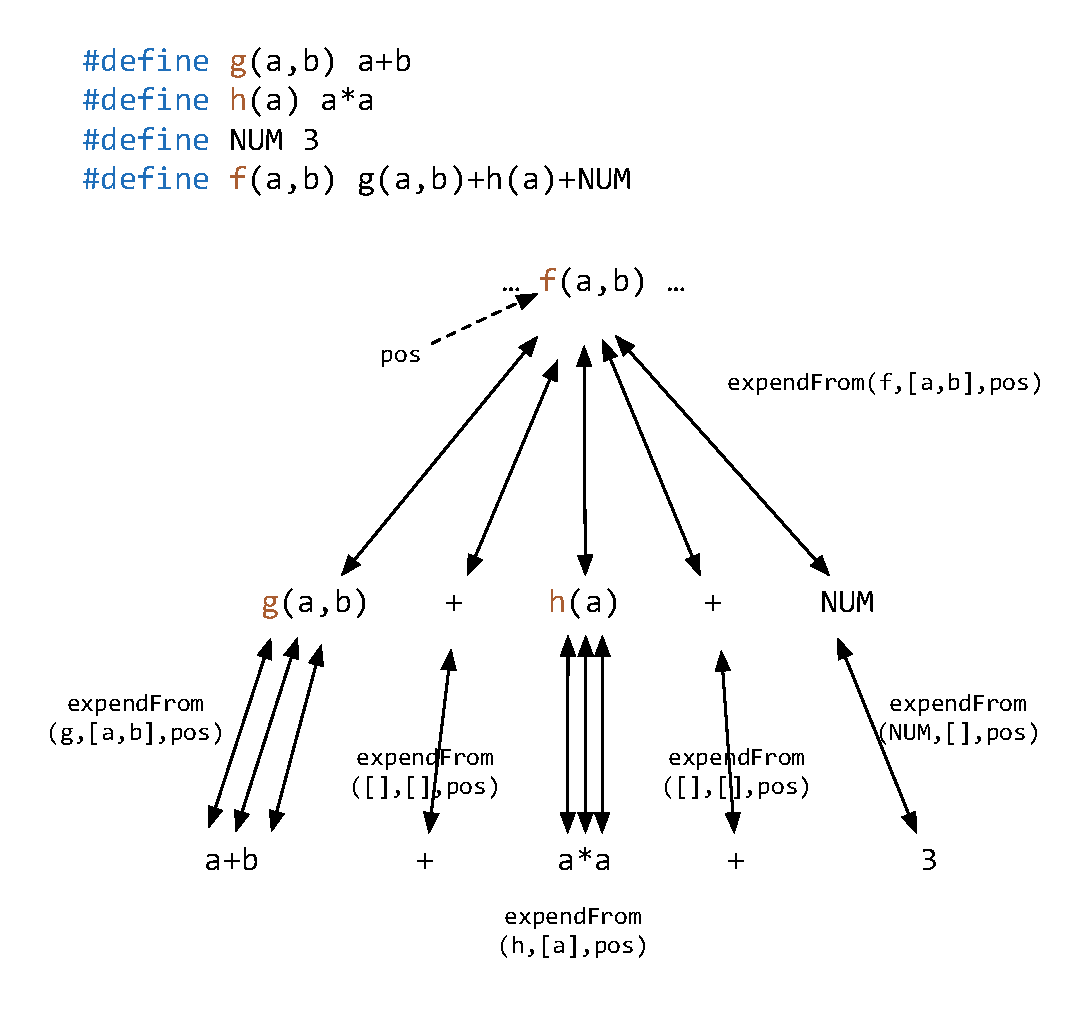
\includegraphics[width=9cm]{pics/original.eps}
\caption{数据结构示例}
\end{figure}
\label{pic:datastruct}
图~\ref{pic:datastruct}展示了宏定义和宏调用展开后的数据结构。构造过程如下:
\begin{itemize}
\item 预处理器扫描源代码发现宏定义指令,将宏定义及其展开式纪录在数据结构中。
\item 当预处理器扫描到位置 $pos$ 时,根据算法规则3,发现函数式宏(\emph{function-like macro})
  调用,分析参数数量,确认宏调用
\item 确认宏调用后,在 $pos$ 位置建立切分点,认为 $f(a, b)$ 是一个独立代码段单元。
  在实现中,这些单元用$Unit$类及其子类实现
\item 独立对$f(a, b)$递归正向展开。正向展开算法在前文中提到(\ref{alg:forward})。
  纪录展开时响应参数位置。
\end{itemize}

图~\ref{pic:datastruct}中的双向箭头表示了词和代码段单元之间的关联关系。
$expandedFrom$中的三个参数表示在下一层的词在正向展开时的来源。
第一个参数描述了该词来源于哪一个宏定义;
第二个参数描述了展开宏时的参数列表,$[]$ 代表空,即没有参数;
第三个参数描述了顶层宏展开在源代码中的位置。
在本例中,第二层中的 $NUM$ 指向第一层的箭头中,$f$ 表示该词被名为 $f$ 的宏展开,
$[a, b]$表示参数列表, $pos$表示展开在源代码中的位置。

我们可以看到,记录下了这些信息和前文提到的重写步骤的信息
可以互换。因此我们就能在这样的数据结构上
应用我们的反向算法,实现双向预处理器。


\subsubsection{BXCPP框架}
我们基于JCPP实现了自己的双向预处理器BXCPP。所有的项目代码和试验数据都可以
在我们的项目网站\footnote{\url{https://github.com/harouwu/BXCPP}}上找到。
在此我们简介一下BXCPP框架中主要的几个类。
\begin{figure}
\centering
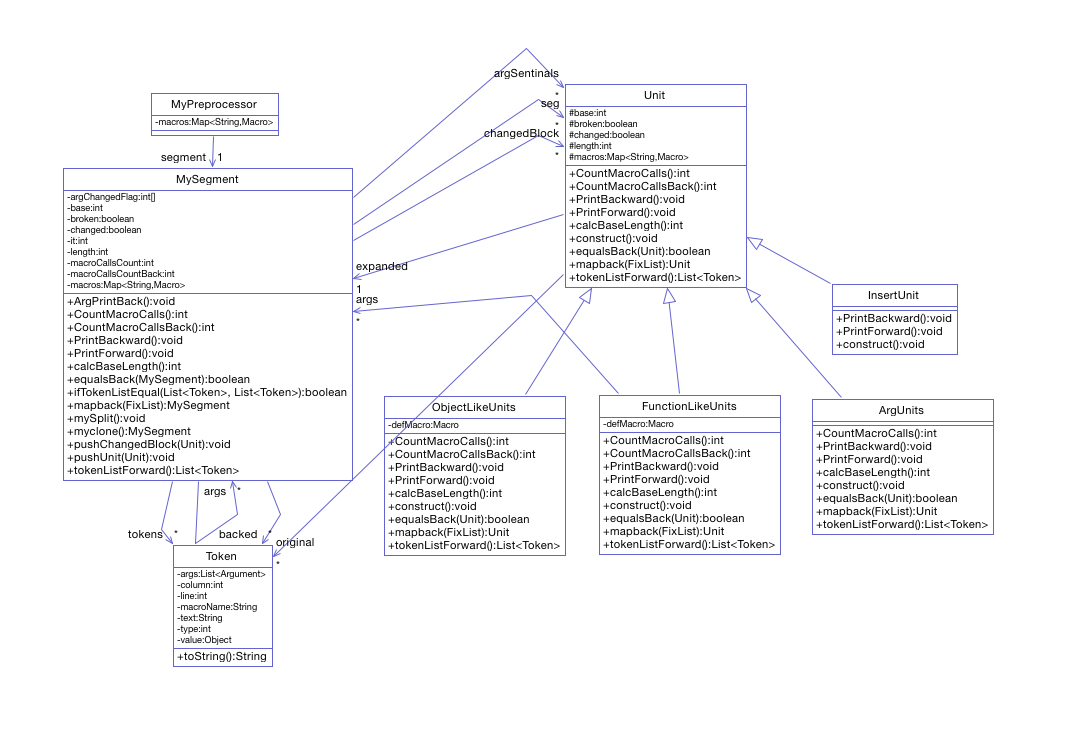
\includegraphics[bb=0 0 1068 746,width=14cm]{pics/class.png}
\caption{主要类类图。}
\end{figure}
\label{pic:classd}

图~\ref{pic:classd}是代码中主要类的类图。小箭头表示包含关系,空心箭头表示继承关系。
我们重写了JCPP中的预处理器 $Preprocessor$类,构造自己的双向C预处理器 $MyPreprocessor$。
该双向预处理器可以识别预处理指令,建立上下文环境纪录和宏定义索引。
同时,双向预处理器把源程序词序列化后,将会把序列保存在类型 $MySegment$里。
$MySegment$封装了词序列和代码段单元序列,同时包含识别拆分代码段单元的函数,类似算法中的$guard$函数。


$Unit$及其子类描述了各种不同类型的代码段单元,他的子类中:
$StringUnit$表示普通文本代码段单元,
$ObjectLikeUnits$表示非函数宏调用代码段单元,
$FunctionLikeUnits$表示函数宏调用代码段单元,
$ArgUnits$表示宏调用参数代码段单元,
$InsertUnit$表示展开式中插入宏参数的代码段单元。

从类图中可以看到,$MySegment$ 和 $Unit$ 类互相包含。
$MySegment$ 中含有 $Unit$ 代码段单元的序列,
而$Unit$在展开时,又包含新的代码段$MySegment$。
这样循环的关系模拟了上一节~\ref{sec:datastruct}中的数据结构,实现了算法。

另外,项目中还定义了许多其他类,如$Token$类描述了词的文本类型等。
具体的项目文档和程序细节,可以访问我们的项目网站了解。
同时我们也实现了前文中提到的 \emph{per-line} 和 \emph{per-file}
两种简单的反向预处理操作。
至此,实现部分基本搭建完成。


\subsubsection{实验基准}
我们的实验在Linux内核版本3.19上执行。我们选择Linux内核源代码因为
Linux是现在最广泛的C语言项目。这之中有许多程序员贡献的代码,包含了不同风格的代码,
也含有大量的预处理指令和宏调用。

为了执行我们的实验,我们需要在Linux内核代码上生成一组修改。
因为我们想看到不同反向预处理算法对程序的影响如何,所以我们需要的修改
应该尽可能出现在有宏调用的函数中。
同时我们在观察中发现,在实际代码中,非函数式宏调用的出现频率
远远高于函数式宏调用。这样导致如果随机生成修改,
大多数修改都会修改非函数式调用,而少数会修改函数式调用。
所以我们根据概率模型,控在非函数式和函数式宏调用的比例为1.5:1。
基于上面的这些计算和宏调用,最终我们从项目中抽取了8000行代码,这之中一共出现了133次宏调用。

接着我们为这抽取的8000行代码生成一组修改。为了模拟现实工程项目中出现的修改,
我们随机性地生成两类修改操作。
第一种是词级别的修改操作,我们随机地替换、删除或插入一个次。
第二种是语句级别的修改,我们随机地删除一句语句、或者从别处随机抽取一句话插入当前位置。
这两种修改的选择是取自现在主流的代码修改工具的方法~\parencite{le2012genprog,QiMLDW14,kim2013automatic}。
其中,GenProg~\parencite{le2012genprog} 和
RSRepair\parencite{QiMLDW14}会直接食用语句级别的修改。
而第一种词级别饿修改则模拟了 PAR~\parencite{kim2013automatic}
中使用的例如替换参数、修改操作符等细微操作。

具体的修改生成过程如下:我们以概率$p$选择在每个词上进行操作。
这个操作可以是插入、替换或删除,三者等概率。
替换操作随机调换一个词中不同字符的位置。
插入操作随机从别处拷贝一个词插入。
类似的,对于每个句子,我们也有味$q$的概率对它生成修改。
修改内容可以是复制或者删除。
复制操作直接把之前一句语句复制过来。
我们根据C语法,根据分号来划分句子。

不同的程序编辑工作会有不同的修改模式:
一个移动工具可能会修改程序中的许多未知,但一个代码修复工具只会修改
程序的少数地方。
为了模拟不同工具之间给出的修改模式,
我们设计了两套不同概率的修改操作集。
一套是高修改密度的操作集合,我们设置$p=0.33$ 和 $q=0.1$。
另一套是低修改密度的操作集合,我们设置$p=0.1$ 和 $q=0.05$。

我们生成了10组修改操作集合,其中5个是高密度的,5个是低密度的。
具体生成的修改数量在表~\ref{tbl:changes}中。
\begin{table}[htbp]
\caption{C实验中生成的修改操作}\label{tbl:changes}
\centering
% \begin{tabular}{|l|lllll|lllll|}
%   \hline
%   Density & \multicolumn{5}{c|}{Low} & \multicolumn{5}{c|}{High} \\
%   \hline
%   Set & 1 & 2& 3& 4 & 5 & 6 & 7 &8 &9 &10\\
%   \hline
%   Changes & 952 & 885 & 956 & 967 & 884 & 3133 & 3136 & 3088 & 3123 &
%                                                                       3048 \\
% \hline
% \end{tabular}
\begin{tabular}{|l|l|lllll|}
  \hline
  \multirow{2}{2cm}{Low Density} & Set & 1 & 2 & 3 & 4 & 5  \\
  \cline{2-7}
                                 & Changes & 952 & 885 & 956 & 967 & 884 \\
  \hline
  \multirow{2}{2cm}{High Density} & Set & 6 & 7 & 8 & 9 & 10 \\
  \cline{2-7}
                                 & Changes & 3133 & 3136 & 3088 & 3123 & 3048\\
  \hline
\end{tabular}
\end{table}

\subsubsection{自变量}
实验中我们认为以下变量是自变量:
(1)\emph{Techniques},我们认为我们的算法和另外两种简单的算法,
per-file和per-line不同。
(2)\emph{修改密度},不同组之间,修改出现的密度不同。我们的实验中同时出现高密度和低密度。

\subsubsection{因变量}
实验中我们认为有两个因变量。
(1)\emph{剩余宏调用的数量}。我们在反向预处理后再次调用正向预处理,
  依次纪录有多少宏调用呗展开。因为实验的方法中没有一种会引入新的宏调用,
  所以纪录下的就是声誉宏调用的数量。
  为了减少包含系统头文件中的宏调用带来的干扰,我们只会记录当前文件中的
  宏调用展开次数。
(2)\emph{错误的数量}。这里的错误是指当我们在反向预处理后再次调用正向预处理,
  比较新生成的预处理后代码和之前应用修改的预处理后代码之间是否不同。
  这里我们使用Unix系统提供的文件比较工作 $fc$。
  每当$fc$给出一处不同时,我们认为是一个错误。
(3)\emph{报错}。我们的方法会检测修改能否被映射回去,
我们对于生成的修改操作集合,我们也会记录报错的数量。


\subsection{影响实验可信度的因素}
一个影响实验外部可信度的因素是我们生成的这些修改操作能不能被一般化为
真实项目中产生的程序修改。
为了减轻该因素的影响,我们使用了从现有工具分析得来的不同类型的修改,
同时控制修改出现的频率,这样可以更好地模拟现实项目中的程序修改。

一个影响实验内部可信度的因素是我们实现的三种双向预处理器可能实现错误。
为了减轻该因素的影响,我们通过在Linux内核,自写测试集上不断修改错误来
保证我们的实现是可信可靠的,不会对实验产生负面影响。

\subsection{实验结果}
\begin{table}[htbp]
  \caption{实验结果}\label{tbl:results}
\centering
\begin{tabular}{|l|l|lllll|}
  \hline
  Low Density & Set & 1 & 2 & 3 & 4 & 5\\
  \hline
  \multirow{3}{*}{Our Approach} &  Macros & 73 & 75 & 72 & 80 & 81 \\
  \cline{2-7}
              &Errors & 0 & 0 & 0 & 0 & 0  \\
  \cline{2-7}
              & Failures & n & n & n & n & n \\
  \hline
  \multirow{3}{*}{Per-Line} & Macros & 23 & 25 & 23 & 20 & 26 \\
  \cline{2-7}
              & Errors & 6 & 7 & 6 & 7 & 7  \\
  \hline
  \multirow{3}{*}{Per-File} & Macros & 0 & 0 & 0 & 0 & 0  \\
  \cline{2-7}
              & Errors & 0 & 0 & 0 & 0 & 0 \\
  \hline
  \hline
  High Density & Set & 6 & 7 & 8& 9& 10\\
  \hline
  \multirow{3}{*}{Our Approach} &Macros & 47 & 51 & 53 & 48 & 44 \\
  \cline{2-7}
              &  Errors & 0 & 0 & 0 & 0 & 0  \\
  \cline{2-7}
              & Failures & n & n & n & n & n \\
  \hline
  \multirow{3}{*}{Per-Line} & Macros & 9 & 7 & 7 & 8 & 10  \\
  \cline{2-7}
              & Errors & 6 & 6 & 7 & 6 & 6 \\
  \hline
  \multirow{3}{*}{Per-File} & Macros & 0 & 0 & 0 & 0 & 0  \\
  \cline{2-7}
              & Errors & 0 & 0 & 0 & 0 & 0 \\
  \hline\end{tabular}
\\
\parbox{\columnwidth}{ \ \\
\footnotesize ``Macros'' 行表示剩余的宏调用数量。``Errors'' 行表示修改造成的错误数量
      ``Failure'' 行表示反向预处理器发生了多少错误。}
\end{table}

% \begin{table*}[htbp]
% \caption{Macros remainings and errors of different algorithms and data set}
% \centering
% \begin{tabular}{l|cc|cc|cc}
% \hline
% Algorithm  &High Mutation & &Low Mutation & &Average &  \\
%  &Remain &Error &Remain &Error &Remain &Error \\
% \hline
% CPP-TRANS &120 &0 &243.8 &0 &181.9 &0 \\
% PER-FILE &0 &0 &0 &0 &0 &0  \\
% PER-LINE &25.6 &5.8 &64.2 &2.4 &44.9 &4.1 \\
% \hline
% \end{tabular}
% \end{table*}

我们实验的结果在表~\ref{tbl:results}中。
接着我们将会讨论本章开始时提到的三个研究问题的解答。 

\subsubsection{研究问题1} 我们从表中可以看出,我们的方法尽可能地保存了宏调用。 
Per-line方法保留了一些宏调用,而per-file方法,不出所料的,完全不
保留宏调用。我们进一步考察了为什么per-line方法保存了这么少的宏调用。
其中一个主要原因是我们发现在Linux内核代码中,时常出现一行中有多个宏调用
的情况。而一旦修改发生在该行,
per-line方法会破坏该行中的所有宏调用。
\subsubsection{研究问题2} 从表中看出,我们的方法和per-file方法都不会产生错误。
但per-line方法产生了一些错误。我们认为这是因为存在一些宏调用形式是多行
宏调用。这些宏调用的参数一般是一个表达式,甚至一个句子,以至于一行中
无法写完而需要换行。
\subsubsection{研究问题3} 正如之前讨论过的,我们的方法会在反向变换时对
不合适的修改操作进行报错。这是因为有时一个修改会意外地在预处理后的代码中引入一个新的宏调用。
这样就无法满足正确性性质的PUTGET性质。
但是,在我们的实验中没有看到类似的情况。
这是因为宏定义的名字之间差别比较大,而宏调用的位置在整个代码中很零散,通过调换字符位置或者拷贝
并不能引入不合适的修改操作。
同时我们知道另外两种方法并不能检测这种不合适的修改操作,
所以在表~\ref{tbl:results}关于报错的部分都留空了。

尽管出现不合适的修改操作而导致报错的情况在实际工作中也不常见,
但理论上我们的方式是可以对这种情况作出报错的。

%另外理论上我们的方式可以能会出现误报情况:
%我们的算法报错但是存在一种映射修改的方式。
%比方说我们考虑以下代码:
%\begin{lstlisting}
%#define p (x)
%plus p
%\end{lstlisting}
%$plus$是在之前的代码段~\eqref{eqn:expansion}中定义的宏。
%在预处理后这段代码会展开成$plus\ (x)$。
%如果我们把最后的括号拆分成$)\ hello$,那么这个修改会使得我们的方法报错

%Although probably being rare in practice, theoretically our approach
%may report false alarms: our approach reports a failure but
%a correct change on the source program exists. {For example, let consider the
%  following code piece,
%\begin{lstlisting}
%#define p (x)
%plus p
%\end{lstlisting}
%where $plus$ is the macro defined in code
%piece~\eqref{eqn:expansion}. After preprocessing, this code piece becomes
%$plus\ (x)$. If we change the last parenthesis into $)\ hello$, our
%approach reports a failure because first $p$ will be expanded and then
%the expanded content forms a new macro invocation with $plus$.
%However, there exists a feasible change: replacing $p$ with $hello\ p$.}
%\end{comment}

%%% Local Variables:
%%% mode: latex
%%% TeX-master: "main"
%%% End:
